\chapter{Structural Analysis of QoE Problems}
\label{ch:measurement}

We have seen that the limitations of prior approach have caused 
pervasive QoE problems in the wild (Chapter~\ref{ch:related}),
and this dissertation seeks to improve QoE by exploring a 
new data-driven approach which leverages the QoE information 
observed by millions of sessions in real time (Chapter~\ref{ch:overview}).
The key insight to make such data-driven QoE optimization practical
is the observation that there are {\em persistent structures in the 
QoE-determining factors} (Section~\ref{sec:overview:unifying}).

In this chapter, we provide more empirical evidence of these persistent
structures using a large-scale structural analysis on the 
QoE problems of Internet video and Internet telephony.
In particular, we shed light on the spatial criticality and 
temporal persistence of these structures of QoE-determining factors.
To this end, our analysis focuses on the spatial and temporal patterns
of QoE problems.
\begin{itemize}

\item {\em Temporal patterns:} 
Is each QoE problem a transient for 
a specific ISP, CDN, or provider (or combination of these) or are 
these problems persistent over long periods?

\item {\em Spatial patterns:} 
Are the QoE problems uniformly spread through the 
space of feature combinations or are there specific 
combinations that have a higher concentration?

\end{itemize}
In addition, we also show there are substantial correlations
among the QoE problems of different metrics, suggesting that
it is possible to improve multiple QoE metrics simultaneously.

This chapter is organized as follows. 
Section~\ref{sec:measurement:video} presents the structural analysis
on video QoE,
Section~\ref{sec:measurement:voip} presents a similar analysis on 
VoIP QoE, and Section~\ref{sec:measurement:summary} summarizes
the chapter with key observations.


%The key role that QoE plays in impacting user engagement,
%and consequently providers' revenues, has motivated recent
%efforts, including this dissertation, in improving the QoE of 
%Internet applications like
%Internet video and Internet telephony.
%Before we embark on designing and deploying new 
%schemes to improve QoE, we need to first understand 
%the nature of QoE problems.
%To this end, this section uses large-scale datasets collected
%from real users to shed light on the structure of today's 
%QoE problems  in the wild.
%In particular, we observe that 
%(1) a substantial fraction of video and VoIP 
%sessions suffer from QoE problems; and
%(2) QoE problems exhibit patterns both 
%spatially (e.g., correlation to
%certain client-side features) and temporally
%(e.g., prevalent/persistent quality issues).
%
%This chapter is organized as follows.
%Section~\ref{sec:measurement:video} presents a 
%measurement study on video QoE.
%Using 300 million video sessions collected over a 
%two-week period, we show how severe today's
%QoE problems are, and  analyze the spatial
%and temporal properties of these QoE problems.
%Section~\ref{sec:measurement:voip} presents
%a similar measurement study on Internet telephony 
%QoE based on a dataset from one of the most 
%popular VoIP  service providers.
%Finally, Section~\ref{sec:measurement:summary} 
%summarizes the chapter with key findings 
%which motivate the ideas proposed in later 
%chapters.


\section{Internet Video}
\label{sec:measurement:video} 

\newcommand{\numsessions}{numsessions\xspace}
\newcommand{\problemsession}{problem session\xspace}
\newcommand{\problemsessions}{problem sessions\xspace}
\newcommand{\cluster}{cluster\xspace}
\newcommand{\clusters}{clusters\xspace}
\newcommand{\problemcluster}{problem cluster\xspace}
\newcommand{\problemclusters}{problem clusters\xspace}
\newcommand{\problemratio}{problem ratio\xspace}

\newcommand{\criticalcluster}{critical cluster\xspace}
\newcommand{\criticalclusters}{critical clusters\xspace}

%In this section, we begin by describing our dataset and
%metrics under consideration.
%Then we present preliminary statistics on today's 
%video QoE to motivate 
%the types of structural insights we would
%like to obtain regarding the nature of video 
%quality problems. 
In this section, we begin by describing our dataset and
the methodology of analyzing spatial and temporal patterns
of video QoE problems 
(Section~\ref{subsec:measurement:video:method}),
then present our results in 
Section~\ref{subsec:measurement:video:spatial},
~\ref{subsec:measurement:video:temporal}, and
~\ref{subsec:measurement:video:correlation},
and finally summarizes the observations in 
Section~\ref{subsec:measurement:video:discuss}.

\subsection{Methodology}
\label{subsec:measurement:video:method}

\mypara{Dataset}
We use the same dataset as described in 
Section~\ref{subsec:related:video-qoe}. 
The dataset consists of client-side measurements of
video  quality from over 300 million sessions of 
379 distinct content providers spanning diverse
genres, both live and video-on-demand content, different
content delivery platforms, different types of  bitrate adaptation
algorithms, and device/browser platforms.

\mypara{Session-level features}
The basic unit in our dataset is a video session. 
A session represents a user viewing a video on one of 
our affiliates' sites for some duration of time.
Each session is associated with a set of \emph{seven 
features}: 
\begin{packedenumerate}
\item \emph{ASN:} The Autonomous System Number 
(ASN) that the client IP belongs  to. 
Note that a single ISP (e.g., Comcast) may own 
different ASNs both  for management and business reasons. 
We focus on the ASN as it is more fine-grained
than the ISP granularity.  We observe in aggregate 
15K unique ASNs spanning multiple countries. 

\item \emph{CDN:}   In total, we observe 19 unique CDNs 
spanning popular CDN providers as well as several in-house 
and ISP-run CDNs. (Some providers use proprietary 
CDN switching logic; in this case we pick the segment of 
the session with the CDN used for the longest
duration.)


\item \emph{Content provider (Site):} This is the specific 
provider from which the client requested some content. 
We have  379 content providers that span different 
genres of content.  We use the terms site and
content provide interchangeably.

\item \emph{VoD or Live:} Video  content  falls in one 
 of two categories: video-on-demand (VoD) or Live.  
 We use a binary indicator to see if the particular
  content was a Live event or a 
 VoD video. 


\item \emph{Player type:} We see diverse  players 
such as  Flash, Silverlight, and HTML5.

\item \emph{Browser:} We see diverse client browsers 
including Chrome, Firefox, MSIE, and Safari. 

\item \emph{Connection type:} Finally, we  have the 
type of access network connection such  as
 mobile/fixed wireless, DSL, fiber-to-home. 
These annotations come from third party services~\cite{quova}.
 
\end{packedenumerate}

%Now that we see that many video sessions suffer from bad QoE, 
%we would like to know whether there is any patterns of these 
%video quality problems.
%In particular, we are interested in the temporal and spatial patterns 
%of QoE problems:
%\begin{itemize}
%\item Temporally, is each problem a transient or one-off event for 
%a specific ISP, CDN, or provider (or combination of these) or are 
%these problems persistent over long periods?
%\item , are the problems uniformly spread through the 
%space of feature combinations or are there specific 
%combinations that have a higher concentration?
%\end{itemize}

\mypara{Identifying problem sessions} 
Our focus  is on understanding quality problems as they appear 
in the wild. 
To this end, we identify \problemsessions w.r.t. each of the 
quality metrics. Note that a given session may appear as a 
\problemsession on a subset of  metrics; i.e., it might have a low
join time but may have a high buffering ratio or vice versa. 
We consider the  metrics separately to avoid implicitly 
assuming that the metrics or failures are correlated.

\begin{packeditemize}
\item For join failures, we use a binary indicator if the 
session failed or not.  
For the remaining metrics, we choose specific 
thresholds based on domain-specific
knowledge and observations in prior work\footnote{
We do acknowledge that there is no ideal choice of 
threshold and it is likely that these thresholds will evolve 
as user expectations and network conditions improve. 
As such, the choice of thresholds is illustrative of the 
structure of video quality problems that occur today. 
The methodology and qualitative observations we 
present are not  tied to the  specific  thresholds.
We have confirmed that the results are qualitatively 
similar for other choices  of these thresholds as well. }.  
Our specific thresholds and rationale are follows.
\item For buffering ratio, we identify a \problemsession 
if the value is greater than 5\%; this is based on the 
observation that beyond this value there is a sharp 
decrease in amount of video viewed~\cite{sigcomm11}.  
\item For bitrate, we mark a \problemsession if the average
bitrate is less than 700kbps; this value roughly
 corresponds to the recommended ``360p'' setting on 
 video providers. 
We use a fixed threshold of bitrate in this work for 
simplicity, but we do acknowledge that bitrate settings 
are content-dependent (e.g., some contents do not provide 
high resolution streams).
\item Third,  we mark all sessions with a join
time greater than 10 seconds; this represents a 
conservative upper bound on the
tolerance of users~\cite{webhci1,akamai-imc12}.  
\end{packeditemize}

\mypara{Identifying problem clusters}
 We begin by dividing our dataset into discrete one 
 hour epochs.\footnote{One hour is the finest 
 granularity of the dataset and thus we cannot 
 analyze effects at smaller timescales.} As a
first step to analyze the structure, we 
\emph{cluster}\footnote{The term ``cluster'' represents a 
group of sessions that share common features, and it is 
indeed  different from traditional   clustering algorithms 
where a cluster can be a group of any data points.} 
together sessions that share one or more client/session 
features within the same epoch.   
For instance, the \cluster ``ASN=$\mathit{ASN1}$'' describes 
all sessions where the user belongs
to $\mathit{ASN1}$ and the cluster 
``ASN=$\mathit{ASN1}$, CDN=$\mathit{CDN1}$'', 
describes all sessions where the
user belongs to $\mathit{ASN1}$ and the session was 
assigned to a server from $\mathit{CDN1}$.
In order for our observations to be reliable, 
we want to focus on  clusters that are deemed to be 
statistically significant sources of problem sessions. 
To this end, we define the \problemratio of a
cluster as the ratio 
$\frac{\textrm{\# of \problemsessions}}{\textrm{\# of
sessions}}$. Then, we cull out the \clusters whose 
\problemratio is
significantly higher than the global average \problemratio.  
We also remove all \clusters that have a small number 
of sessions in aggregate; i.e., problems observed within a 
small cluster may not be statistically significant.
Combining these two steps, we define a \problemcluster 
as a \cluster that has a \problemratio $\geq 1.5 \times$ the
global \problemratio,\footnote{This value roughly represents 
two standard deviations away  from the mean of the
per-cluster \problemratio distribution.}  and the number of 
sessions in this cluster is $\geq1000$.  
In the rest of this paper, we start from the \problemclusters 
as our basis and subsequently refine the analysis.

 
\begin{figure}[t!]
\centering
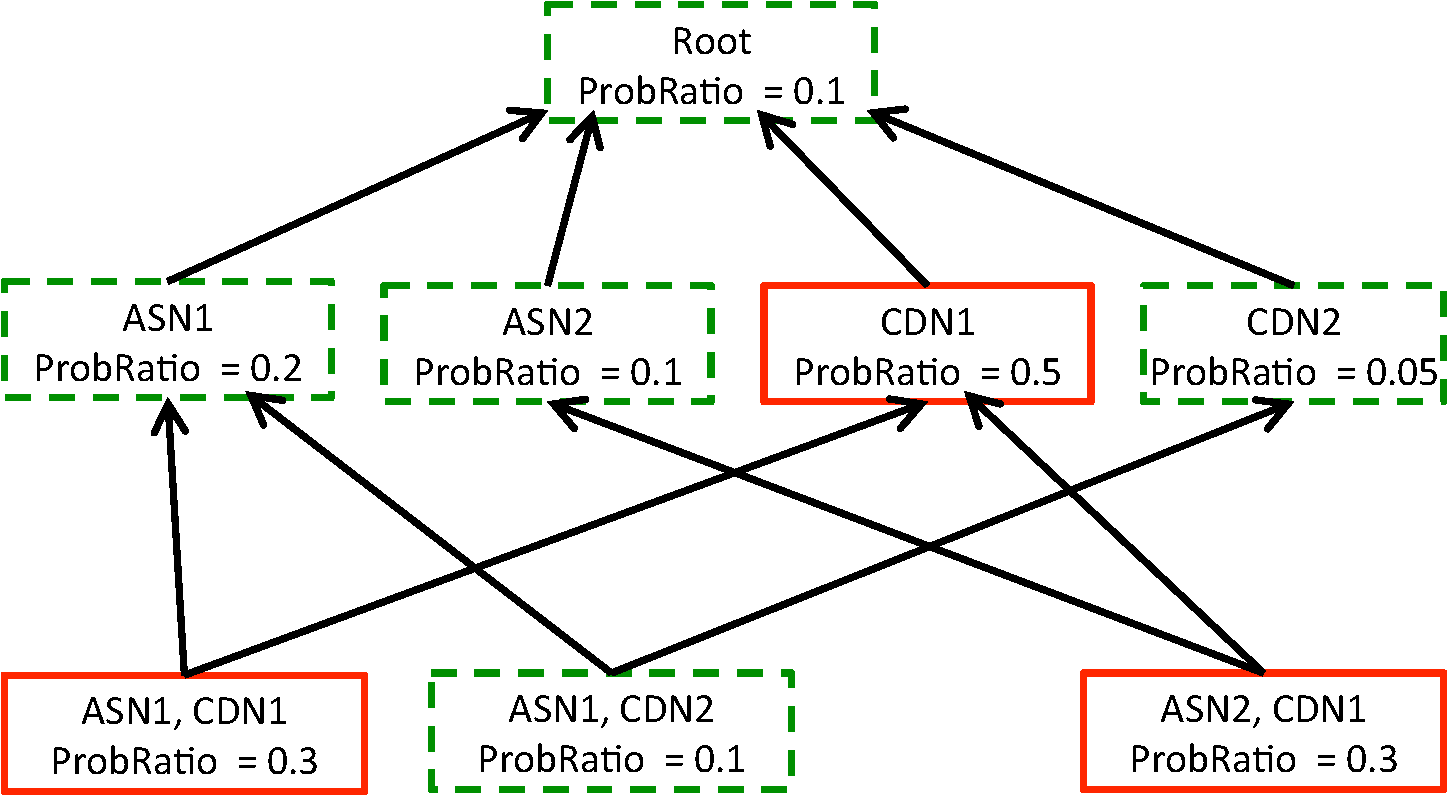
\includegraphics[width=0.7\textwidth]{figures/conext13-criticalcluster.pdf}
%\vspace{-0.3cm}
\caption{Representing the relationship between clusters using a DAG.  
Red boxes represent the \problemclusters.
%The dashed-green boxes show clusters without a high \problemratio and the solid-red boxes identify the \problemclusters.
}
\label{fig:method:critcluster}
\end{figure} 

%\begin{figure*}[t]
%\centering
%\captionsetup[subfigure]{justification=centering,farskip=-1pt,captionskip=5pt}
%\subfloat[Representing the relationship between clusters using a DAG.  
%Red boxes represent the \problemclusters.
%%The dashed-green boxes show clusters without a high \problemratio and the solid-red boxes identify the \problemclusters.
%]{
%   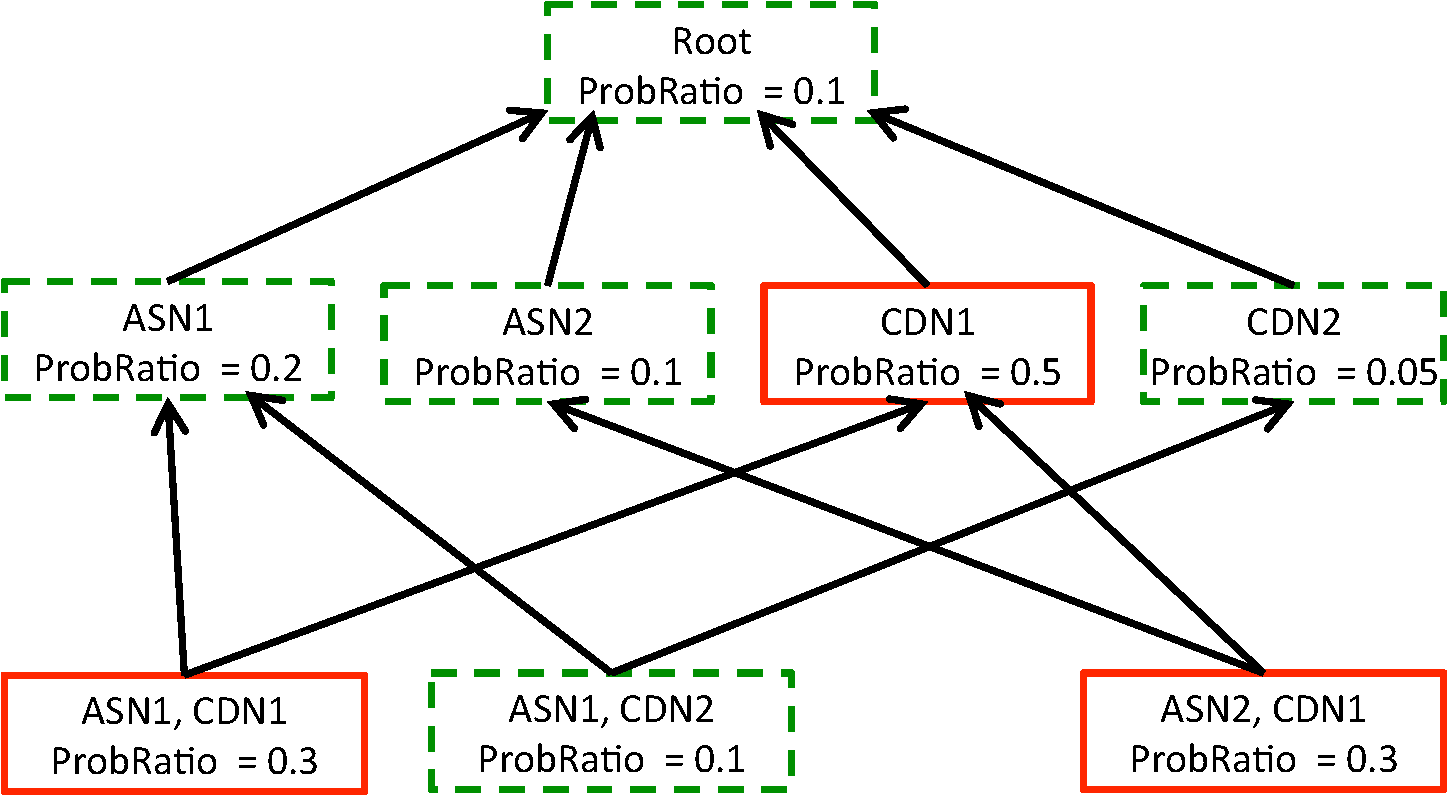
\includegraphics[width=0.6\textwidth] {figures/conext13-criticalcluster.pdf}
%   \label{fig:method:critcluster}
% }
%% \hspace{0.4cm}
%\\
%\subfloat[An illustration of the phase transition idea for  identifying a \criticalcluster. 
%%Intuitively,  removing any one feature from this \criticalcluster will cease to 
%%be a \problemcluster and adding any feature  to it will continue to be a \problemcluster.
%]{
%   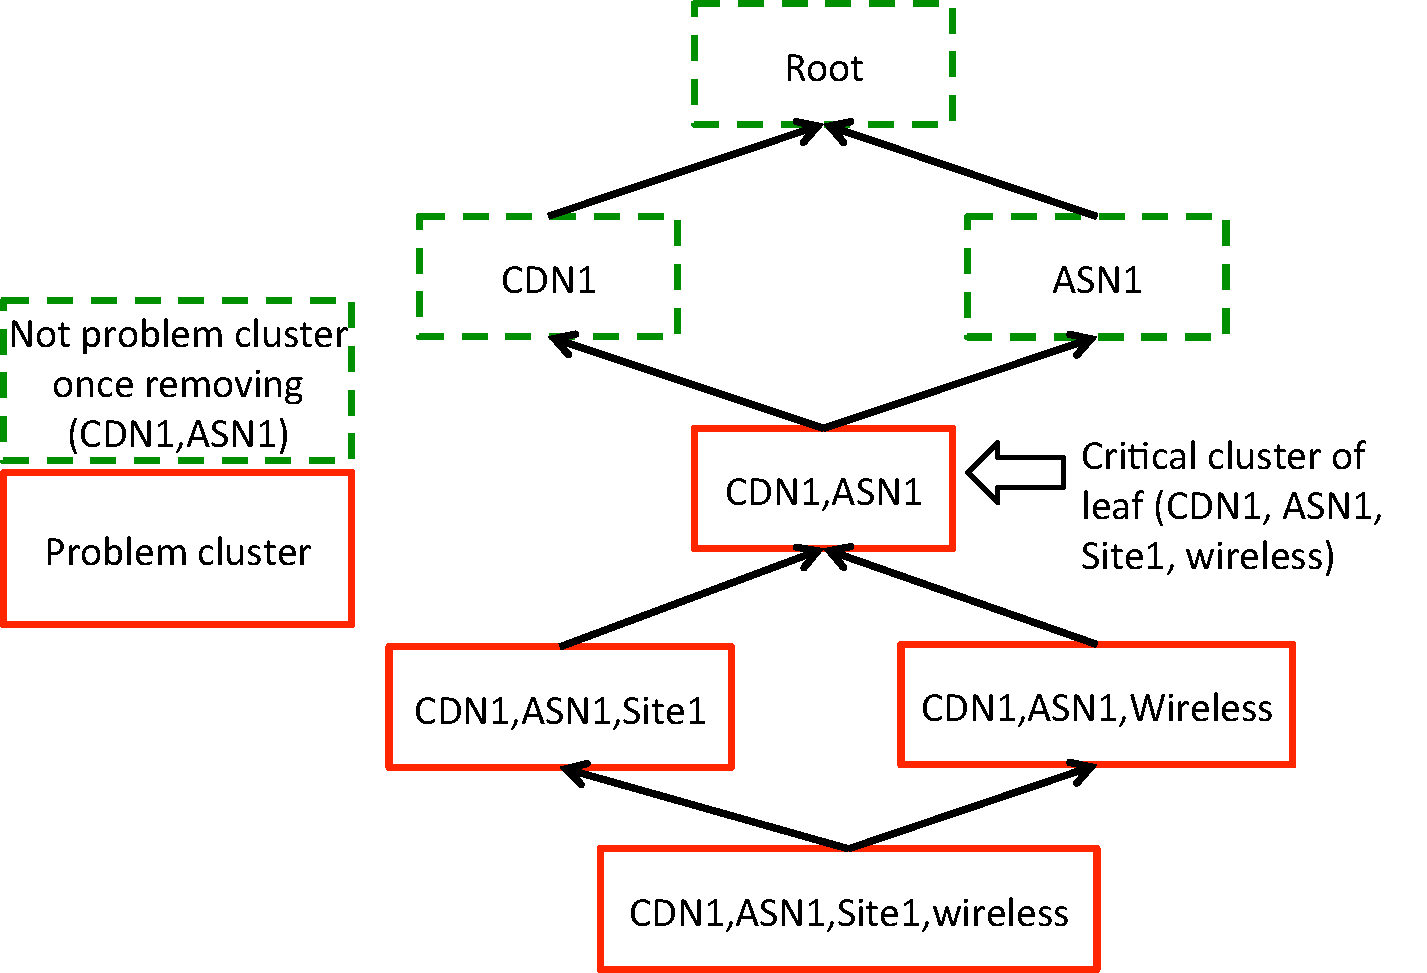
\includegraphics[width=0.6\textwidth] {figures/conext13-criticalcluster_example.pdf}
%   \label{fig:method:critclustr2}
% }
%\caption{Illustrative examples of how to identify \criticalclusters from \problemclusters.}
%\label{fig:pattern:method}
%\end{figure*}

While the grouping of problem sessions into \problemclusters  
provides some insights into the structure of problems, 
there is still one key missing aspect. 
Specifically, we may have different granularities of \problemclusters
that may be intrinsically related to the same underlying root cause.
Thus, our next step is to refine these \problemclusters to identify such
potential causal structures across the \problemsessions. 

The set of all \clusters can be viewed as a \emph{hierarchical}
structure across the space of client/session features 
 with natural parent-child relationships. We can visualize
these parent-child relationships as a DAG as shown in 
Figure~\ref{fig:method:critcluster}.  
A cluster $\mathit{C1}$ is a parent of cluster $\mathit{C2}$, 
if the set of features defining the  cluster $\mathit{C1}$
is a strict subset of that of $\mathit{C2}$. 
For instance, the  cluster ``$\mathit{ASN1}$'' is a parent of
the more specific clusters ``$\mathit{ASN1}$, $\mathit{CDN1}$'' 
and   `` $\mathit{ASN1}$, $\mathit{CDN2}$''. 


\mypara{Identifying critical clusters}
Our goal is to identify a small number of {\em \criticalclusters} 
that can potentially explain the occurrences of different 
\problemclusters.  
In our example in Figure~\ref{fig:method:critcluster}, intuitively 
we should pick the ``$\mathit{CDN1}$'' cluster rather than pick 
``$\mathit{ASN1}$, $\mathit{CDN1}$'' and ``$\mathit{ASN2}$, 
$\mathit{CDN2}$'' clusters separately.
Given that we do not have ground truth, \criticalclusters can 
serve as  starting points for further investigation. 
%
An intuitive criterion for  identifying a \criticalcluster is 
analogous to the notion of the minimum description length 
(or Occam's razor) from the machine learning literature. 
Conceptually, we should pick the most  compact description
to explain an observation.  Building on the above intuition, 
we can identify a \criticalcluster as consisting of the minimal 
set of features that when combined together can lead to 
significantly high problem ratio in its \cluster
(e.g., a \problemcluster) and removing even one feature
 from this set will reduce the problem ratio. 
To this end, we identify \criticalclusters using a \emph{phase
transition} algorithm as follows. 
For each session, we construct all logical paths in the DAG 
from the root to the leaf.  
Then, for each of these paths, we identify the point closest 
to the root along this path such that every cluster that is a 
descendant  is a \problemcluster and once removing it every 
cluster that is an ancestor is not a \problemcluster.
We use Figure~\ref{fig:method:critclustr2} to explain the intuition. 
In this figure, ``$\mathit{CDN1}$, $\mathit{ASN1}$'' is the 
\criticalcluster---every cluster that is a child of
this combination is a \problemcluster and if we remove the 
sessions in this combination, the parents ``$\mathit{CDN1}$'' 
and ``$\mathit{ASN1}$'' cease to be \problemclusters.
That is, this combination of features represents a key 
``transition point'' in this hierarchy between \problemclusters 
and non-problem clusters. 



\begin{figure}[t!]
\centering
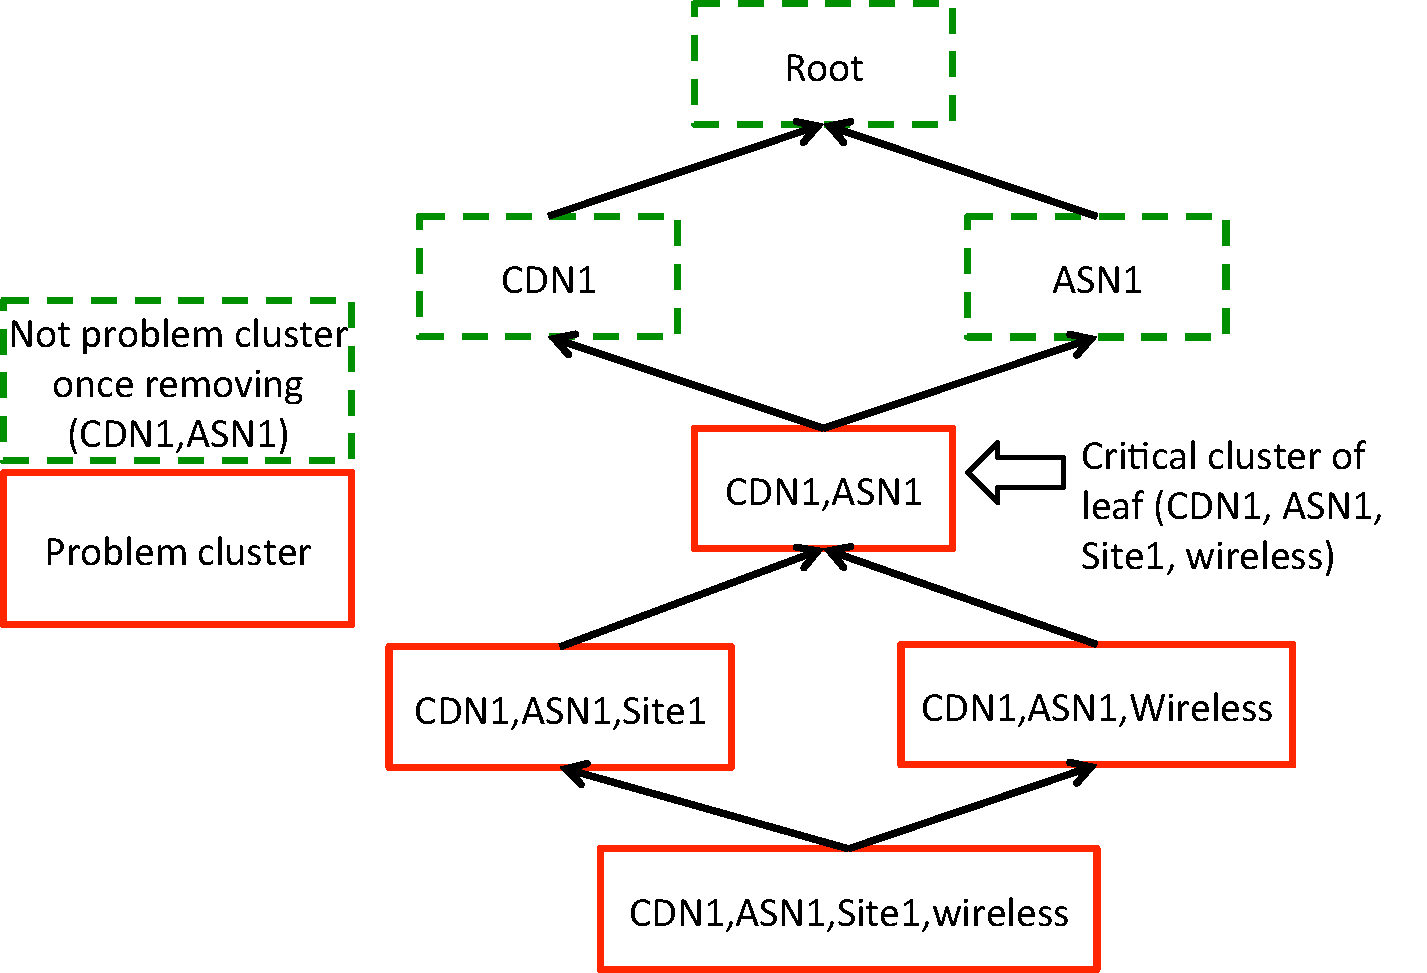
\includegraphics[width=0.7\textwidth]{figures/conext13-criticalcluster_example.pdf}
%\vspace{-0.3cm}
\caption{An illustration of the phase transition idea for  identifying a \criticalcluster. 
%Intuitively,  removing any one feature from this \criticalcluster will cease to 
%be a \problemcluster and adding any feature  to it will continue to be a \problemcluster.
}
\label{fig:method:critclustr2}
\end{figure} 

\subsection{Temporal Patterns}
\label{subsec:measurement:video:temporal}

We begin by analyzing the temporal \emph{prevalence} and 
\emph{persistence} of the \problemclusters.

\mypara{Prevalence of \problemcluster} 
We define the \emph{prevalence} of a \problemcluster as the 
fraction of the total number of epochs in which this cluster 
appears as a \problemcluster.  
% Consider the example in Figure~\ref{fig:method:temporal} with a
%total of 6 epochs, the prevalence of the cluster ``$ASN1$, $CDN1$'' is
%$\frac{4}{6} = 0.67$ and similarly the prevalence of the cluster ``$CDN2$'' is
%$\frac{5}{6} = 0.83$.  
Figure~\ref{fig:measure:prevalence} shows the distribution of 
the prevalence of the \problemclusters for the different
quality metrics. We see a consistent pattern  across all quality 
metrics that around 10\% of the clusters have a prevalence 
greater than 8\% across all metrics. 
In other words, many of these \problemclusters are repeated 
observations that are recurrent problem events. 

\mypara{Prevalence of \problemcluster}
We define the \emph{persistence} of a \problemcluster in terms 
of the length of the consecutive occurrences of this cluster as a
\problemcluster.  
To this end, we coalesce consecutive occurrences of the cluster 
into a single logical event that lasts for multiple hours. 
For each \problemcluster, we  consider the distribution of the 
length of these ``streaks'' and report the median value.
%\emph{median}  and the \emph{maximum}  value. 
%For the timeseries in Figure~\ref{fig:method:temporal}, the ``$ASN1$,$CDN1$'' cluster
%has a median and maximum persistence of 2 while the ``$ASN2$'' cluster has a
%maximum persistence of 4. (In this simple series, the median and max coincide,
%but more generally they will not.)
Figure~\ref{subfig:measure:persistence-median} shows 
the distribution of the median persistence. 
For three of the metrics, more than 60\% of the \problemclusters 
have a median duration that last more than 2 hours.



\begin{figure*}[t]
\centering
\hspace{-1.5cm}
\captionsetup[subfigure]{justification=centering,farskip=-1pt,captionskip=5pt}
\subfloat[Distribution of the prevalence of  \problemclusters]{
   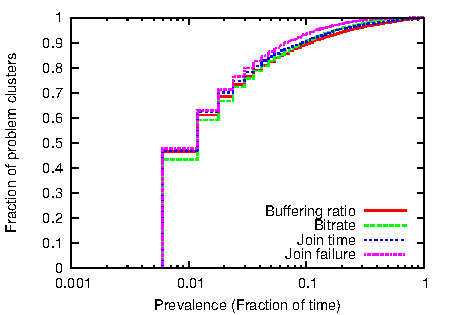
\includegraphics[width=0.52\textwidth] {figures/conext13-figure-cdf-sc-prevalence.pdf}
   \label{fig:measure:prevalence}
 }
\hspace{-0.5cm}
\subfloat[Inverse CDF of the median persistence of \problemclusters]{
   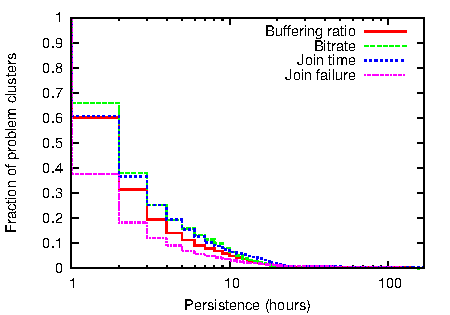
\includegraphics[width=0.52\textwidth] {figures/conext13-figure-cdf-sc-persistence-median.pdf}
   \label{subfig:measure:persistence-median}
 }
 \hspace{-1.5cm}
\caption{Distributions of the prevalence and persistence of  \problemclusters.
We find a natural skewed distribution with a few 
 clusters having high prevalence. 
 Many \problemclusters last multiple hours and that a non-trivial 
 number of \problemclusters last for tens of hours.}
\label{fig:}
\end{figure*}

\subsection{Spatial Patterns}
\label{subsec:measurement:video:spatial}

The previous results showed that there are a non-trivial 
number of persistent/prevalent \problemclusters that last for
several hours. 
As we discussed earlier,  multiple \problemclusters may 
be implicitly related by a single root cause as we saw in
Figure~\ref{fig:method:critcluster}.  
To this end, we focus next on the \criticalclusters using the 
algorithm described in 
Section~\ref{subsec:measurement:video:method}. 
Recall that every  \criticalclusters is also a \problemcluster; 
i.e.,  it has a sufficiently high problem ratio and it has a 
significant number of sessions. The motivation to focus on 
a few critical cluster rather than all \problemclusters is the 
observation (as shown shortly) that a small fraction of 
\problemclusters cover most of the \problemsessions.

\begin{figure}[t]
\centering
   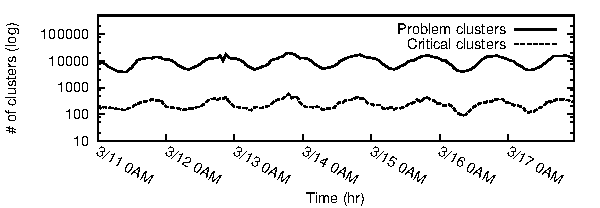
\includegraphics[width=0.7\textwidth] {figures/conext13-time-cluster-count-join-time.pdf}
%\vspace{-0.3cm}
\caption{The number of \criticalclusters is significantly  
smaller than the number of \problemclusters. 
The timeseries shown here  is for the join time; we see 
similar  results for the other quality metrics too.}
\label{fig:critical:reduction}
\end{figure}


\mypara{Critical cluster analysis}
Figure~\ref{fig:critical:reduction} shows the number of 
\problemclusters relative to the number of \criticalclusters 
in the case of the Join Time metric. 
We see that  number of \criticalclusters is almost 
50$\times$ lower than the number of \problemclusters 
suggesting that there are indeed a small number of 
events that might have ``caused''  most  problems.  
One natural question is whether  the \criticalclusters 
\emph{cover} most of the \problemsessions. 
Table~\ref{tab:critical:reduction} summarizes the mean 
coverage and reduction  of the \criticalclusters for the four 
quality metrics and in all cases, we see that the number of 
\criticalclusters is only   2-3\% of the number of 
\problemclusters (i.e., 50$\times$ fewer), but they manage to
cover 44--84\% of the \problemsessions. 
As a point of reference,  we also show the coverage of 
the \problemclusters; i.e., not  all sessions are part of a 
\problemcluster as they may be part of  small clusters or 
clusters with very small \problemratio. 
We see that the \criticalclusters cover almost all 
\problemsessions that are part of some \problemcluster; 
i.e., many of the coverage  gaps are really due to 
\problemsessions that belong to a statistically insignificant 
cluster (i.e., either with too few sessions or with 
too few \problemsessions).
 
 
\begin{table}[t]
\begin{center}
\begin{small}
\begin{tabular}{c|p{2cm}|p{2cm}|p{2.5cm}|p{2.5cm}}
Metric	& Mean \problemclusters & Mean \criticalclusters & Mean \problemcluster coverage & Mean \criticalcluster coverage\\ \hline 
BufRatio	 & 10433 & 286 (2\%) & 0.8 & 0.66 (82\%) \\
JoinTime & 9953 & 247 (2\%) & 0.86 & 0.83 (96\%) \\
JoinFailure & 9620 & 302 (3\%) & 0.87 & 0.84 (96\%)\\
Bitrate & 9437 & 287 (3\%) & 0.57 & 0.44 (77\%)
\end{tabular}
\end{small}
\end{center}
\caption{Reduction via focusing only on \criticalclusters 
and the effective coverage  of the \criticalclusters.}
\label{tab:critical:reduction}
\end{table}


Next, we analyze the structure of the \criticalclusters for 
the different quality metrics. 
First, we analyze the types of  client/session  feature 
combinations that appear frequently in the \criticalclusters. 
Then, we analyze if the different metrics are correlated in the 
\criticalclusters. Finally, we highlight some interesting 
observations  and some hypothesis to explain  
the most prevalent \criticalclusters. 



%\begin{figure}[t]
%\centering
%\captionsetup[subfigure]{justification=centering,farskip=-1pt,captionskip=5pt}
%\subfloat[BufferingRatio]{\label{subfig:measure:pie-bufferingratio}
%   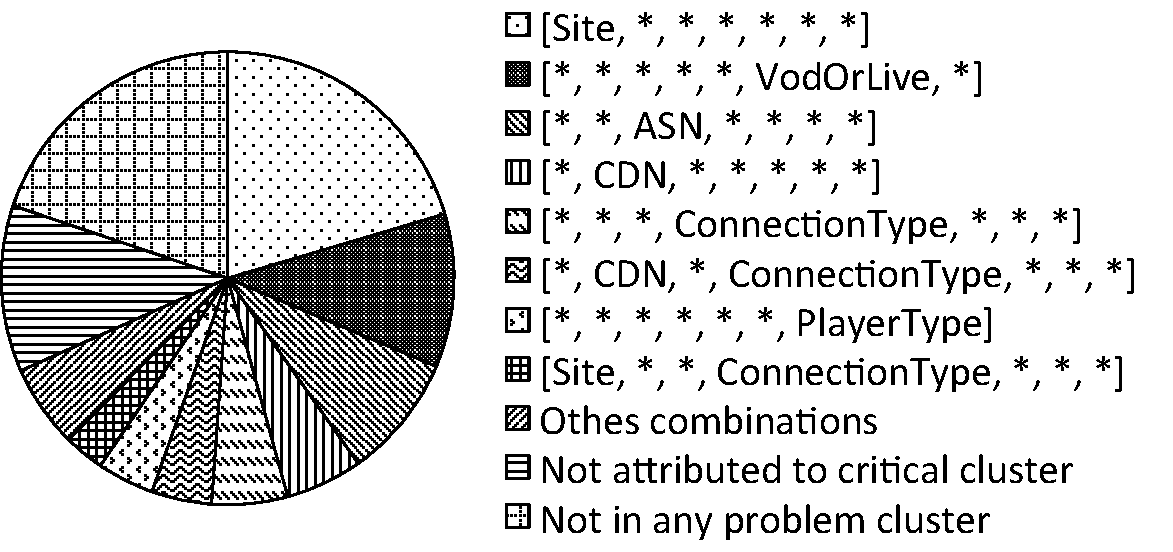
\includegraphics[width=0.48\textwidth] {figures/conext13-figure-pie-bufferingratio.pdf}
% }
%\subfloat[Bitrate]{\label{subfig:measure:pie-bitrate}
%   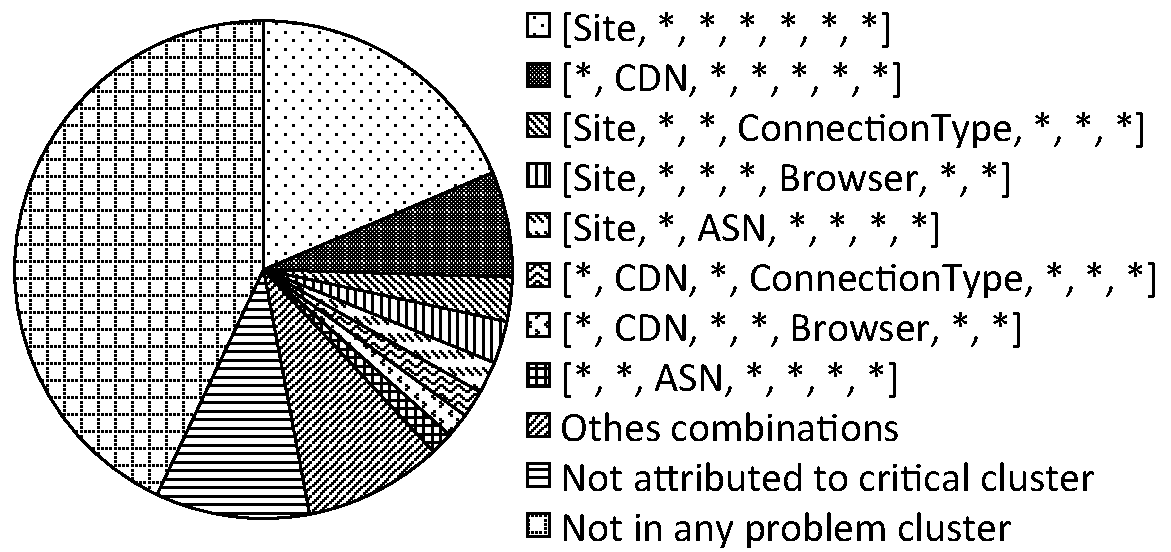
\includegraphics[width=0.48\textwidth] {figures/conext13-figure-pie-bitrate.pdf}
% }\\
%\subfloat[JoinTime]{\label{subfig:measure:pie-jointime}
%   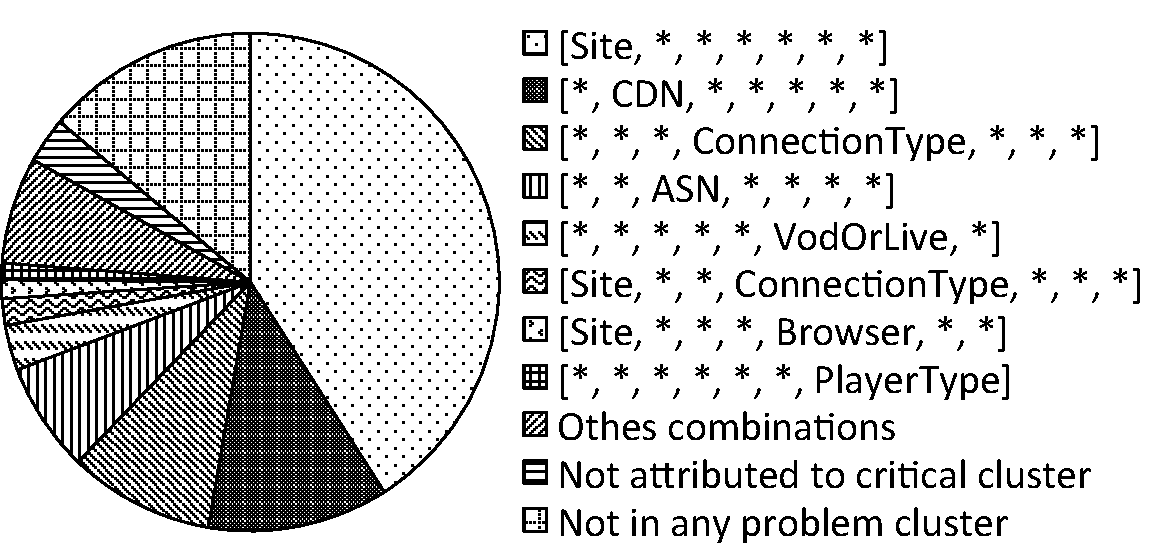
\includegraphics[width=0.48\textwidth] {figures/conext13-figure-pie-jointime.pdf}
% }
%\subfloat[JoinFailure]{\label{subfig:measure:pie-joinfailure}
%   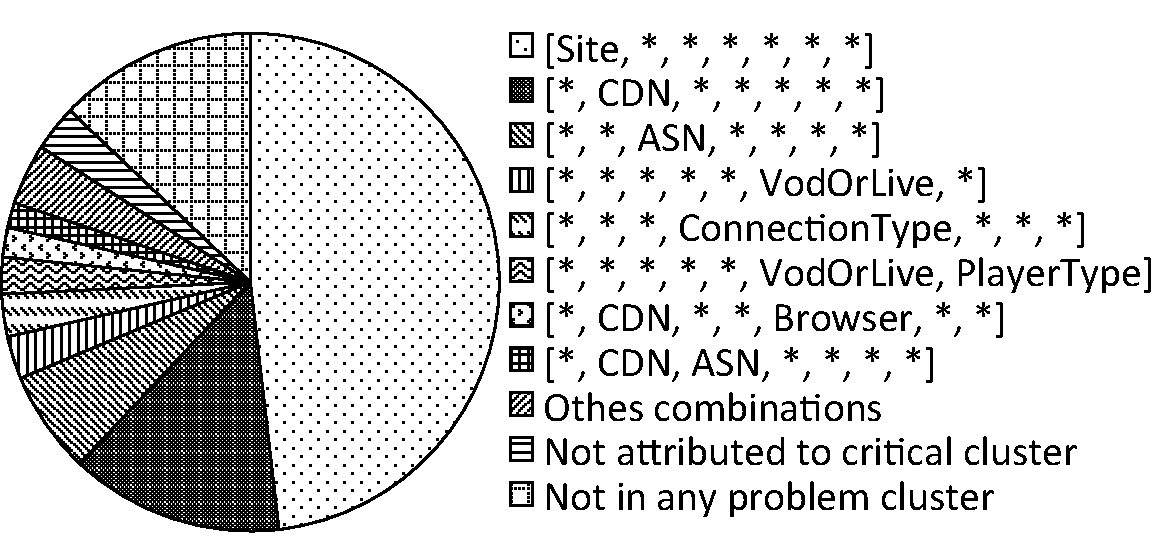
\includegraphics[width=0.48\textwidth] {figures/conext13-figure-pie-joinfailure.pdf}
% }
%\caption{Analyzing the structure of the \criticalclusters.
%The result show a breakdown of the total number of 
%sessions attributed to a specific type of \criticalcluster. 
%Note that there may be multiple values of these features;
%i.e., there can be many Sites and many CDNs  contributing 
%to the Site and CDN sector.}
%\label{fig:critical:pie}
%\end{figure}
%
%\mypara{Types of clusters} 
%Figure~\ref{fig:critical:pie} shows a breakdown of the 
%types of \criticalclusters  for different quality metrics.  
%We aggregate \criticalclusters into the different feature 
%dimension(s) they represent. 
%For instance, if we see a \criticalcluster for $CDN1$ and 
%$CDN2$, we count these toward the CDN contribution 
%in the pie chart.   
%Some \problemsessions may remain unaccounted for 
%in this breakdown for two reasons:
%(a) they are not part of a significant enough 
%\problemcluster or 
%(b) our algorithm did not assign a \criticalcluster for a 
%\problemcluster. 
%This mirrors   the coverage observation we saw earlier in 
%Figure~\ref{fig:critical:reduction}
% and  Table~\ref{tab:critical:reduction}. 
%In almost all cases, most of the unaccounted for sessions 
%fall outside any \problemcluster;  i.e., this is not due to 
%the \criticalcluster detection algorithm. 
%The result shows that the most dominant category of 
%\criticalclusters actually corresponds to a
%\emph{content provider} (labeled as ``Site'').  
%We also see that CDN, ASN, and ConnectionType are
% also prominent types of \criticalclusters across all 
% quality metrics. 
%This suggests that most quality issues are potentially 
%caused by server-side (Site or CDN) or client-side 
%(ASN, ConnectionType) problems rather than a 
%combination (which indicates a bad path between 
%client and server) or other features.

%This is
%related to the coverage observation we saw earlier---with the exception of the
%bitrate category, the coverage is quite high.
 
%Note that this does not mean that the same set of \criticalclusters appear
%across all metrics as we will see next.


\mypara{Understanding most prevalent  \criticalclusters} 
In order to illustrate the causes for the problem,  we 
consider the \criticalclusters with a prevalence higher 
than 60\% for the different quality metrics. 
For clarity of presentation, we only consider the 
\criticalclusters whose features fall in one of the following 
categories: ASN, CDN, Site, and ConnectionType as
our previous breakdown shows these as the most 
dominant features.  
We present this analysis with two disclaimers.  
First, due to the sensitive nature of this data, we do not 
present the names of the actual providers, but focus on their
characteristics.  
Second, this involves a fair amount of manual analysis and
domain knowledge. As such, we intend this result to be 
illustrative (and somewhat speculative) rather than attempt 
to be conclusive.  
This said, we still believe that the high-level insights are 
still useful to inform future video delivery architectures.

Table~\ref{tab:depth} presents some of the anecdotal 
examples we observed.  
The empty cells simply indicate that there were no 
\criticalclusters in this category with a prevalence higher 
than 60\%. 
We see a few interesting patterns here.  
In terms of buffering ratio, we see that the top ASNs are 
typically in Asia, and the content providers that had issues 
typically only had a single bitrate of content. 
The CDNs with buffering/join time problems are also
typically ``in-house'' CDNs run by the Site itself; i.e., 
not a third-party CDN like Akamai or Limelight.  
We also see that wireless connections and wireless
ISPs appear in the buffering and bitrate cells 
respectively, which is somewhat expected. 


One interesting artifact we uncovered in the case of 
join time was that these were mostly ASNs in China 
accessing content from Chinese CDNs but there were
third-party player modules loaded from US providers 
that led to higher join times. Another curious 
observation is that all the Sites with significant join
failures tended to use the same global CDN. 
However, the CDN in aggregate does not have a 
significant presence in terms of failures, except in the 
case of these Sites.\footnote{These Sites used a single 
CDN; recall that our \criticalcluster algorithm will 
prefer more compact descriptions and thus
features these problems to the Site rather than the 
single Site-CDN combination.} 
We speculate that these, presumably low-end, 
providers may have lower priority service and could 
have potentially benefited from using multiple CDNs.


\begin{table}[t]
\begin{center}
\begin{small}
\begin{tabular}{p{1.5cm}|p{3.5cm}|p{2.5cm}|p{3.5cm}|p{2.5cm}}
		& ASN &  CDN   & Site  & ConnType  \\ \hline 

BufRatio	 & Asian ISPs  & In-house, single bitrate   & Single bitrate &  Mobile wireless  \\   \hline
JoinTime 	&  Chinese ISPs accessing CDNs in China, but player loads modules from US CDN	& In-house CDNs of UGC providers & High bitrates  \\  \hline 
JoinFailure 	&   & Same set as buffering ratio & Same single global CDN, maybe low priority providers &  \\ \hline 
Bitrate 	& Wireless provider &   & UGC Sites &    
\end{tabular}
\end{small}
\end{center}
\caption{Analysis of the most  prevalent \criticalclusters. 
A empty cell implies that we found no interesting 
 cluster in this combination.}
\label{tab:depth}
\end{table}


\subsection{Cross-Metric Correlations} 
\label{subsec:measurement:video:correlation}

%We saw in the previous  graph that the types of
% \criticalclusters that contribute the most 
% \problemsessions are very similar across different 
%quality metrics.  
%Note, however, that this does not necessarily mean 
%that the actual set of \criticalclusters are identical. 
%In other words, a different set of CDNs or Sites may 
%be responsible for problems across buffering ratio and
%join time. 
Next, we would like to know how much the \criticalclusters
of different quality metrics correlate with each other.
In other words, a different set of CDNs or Sites may 
be responsible for problems across buffering ratio and
join time. 
To analyze this, we compute the \emph{Jaccard similarity} 
index between the top-100 in terms of the total number 
of \problemsessions covered  \criticalclusters  
for the different metrics. 
(The Jaccard similarity measure for two sets A and B 
is $\frac{|A \cap B|}{|A \cup B|}$.)
We find that the overlap between the different 
metrics is only around 23\% in the best case (buffering 
ratio and join time) and in the worst case is only around
1\% (between bitrate and join failure).  
We manually analyzed the specific clusters and we 
found that  the actual set of Site, CDN, and ASN
\criticalclusters are indeed very different.  

%We look at this in more depth next.
 


%\begin{table}[t]
%\begin{center}
%\begin{small}
%\begin{tabular}{c|c|c|c|c}
%		& Buffering Ratio & Join Time & Join failure & Bitrate \\ \hline 
%Buffering Ratio	 & \fillme & 0.22 & 0.13 & 0.07 \\
%Join Time & \fillme & \fillme & 0.09 & 0.08 \\
%Join failure & \fillme & \fillme & \fillme & 0.008 \\
%Bitrate & \fillme & \fillme & \fillme & \fillme 
%\end{tabular}
%\end{small}
%\end{center}
%\tightcaption{Average Jaccard similarity index between the top-\fillme \criticalclusters for the different metrics. 
% We see that most metrics are relatively uncorrelated, possibly because the 
% critical features are very different.}
%\end{table}

\begin{table}[t]
\begin{center}
\begin{small}
\begin{tabular}{p{2cm}|p{2cm}|p{2cm}|p{2cm}|p{2cm}|p{2cm}}
	BufRatio vs. Bitrate & BufRatio vs. JoinTime & BufRatio vs. JoinFailure & Bitrate vs. JoinTime & Bitrate vs. JoinFailure & JoinTime vs. JoinFailure\\ \hline 
0.07 & 0.23 & 0.13 & 0.08 & 0.01 & 0.09 \\
\end{tabular}
\end{small}
\end{center}
\caption{Average Jaccard similarity index between the top 
100 \criticalclusters for the different metrics. 
 We see that most metrics are relatively uncorrelated, possibly because the 
 critical features are very different.}
\end{table}


\subsection{Key Observations}
\label{subsec:measurement:video:discuss}
%\subsection{Key Observations}

Our key observations from the analysis of \problemclusters 
and  \criticalclusters  are:  

\begin{packeditemize}

\item There is a distinct skewed distribution  in the prevalence; 
around 8-12\% of the \problemclusters appear more than 
10\% of the time.

\item There is also a skewed distribution  in the persistence; 
more than 60\% of  \problemclusters have a median duration 
greater than 2 hours.  

\item We find that a small number of \criticalclusters 
(2-3\% of the number of \problemclusters) can account 
for 44-84\% of all \problemsessions. 

\item While the set of feature combinations in the 
\criticalclusters that cover the most number of 
\problemsessions is very similar across the quality
metrics (i.e., Site, CDN, ASN), the actual values of 
these features is very different (with a max overlap of 23\%). 

\item  We see a few expected patterns  such as Asian 
and wireless ISPs appearing  as most prevalent \criticalclusters. 
We  see some unexpected patterns that can be easily alleviated 
(e.g., the player modules loaded remotely for Chinese users) 
and Sites that could benefit from standard strategies such as 
using more fine-grained bitrates or using multiple CDNs.

\end{packeditemize}





\section{Internet Telephony}
\label{sec:measurement:voip}

We have seen in 
Section~\ref{subsec:related:voip-qoe} that user 
experience is sensitive to poor network performance 
and that a significant fraction of calls suffer from poor 
performance when using \direct routing. 

In this section, we use production data from a large VoIP service 
provide \skype (same dataset described in
 Section~\ref{subsec:related:voip-qoe}) 
to understand the QoE problems in Internet telephony
based on a similar spatial and temporal analysis used in the last section.
We begin by describing the dataset, QoE metrics, and the methodology
of analyzing spatial and temporal patterns
of VoIP QoE problems (Section~\ref{subsec:measurement:voip:method}),
and present our results in 
Section~\ref{subsec:measurement:voip:spatial}, 
~\ref{subsec:measurement:voip:temporal}, and
~\ref{subsec:measurement:voip:correlation}.
%and finally discuss the key takeaways in 
%Section~\ref{subsec:measurement:voip:discuss}
%quantify the impact of network metrics on 
%audio call quality, and patterns of poor network performance. 
%The observations motivate the need for and the design 
%requirements of \hybrid.


%{\em How well does PNR on average values compare to 
%using full packet traces?} 
%Analysis of a subset of ($70$K) calls with full packet traces 
%shows that $80\%$ of calls rated ``non-poor'' using the 
%thresholds on average metrics (``at least one poor metric'') 
%have a (packet-trace based) MOS score higher than 
%three-quarters ($75\%$) of calls rated ``poor'' using the 
%average metrics. We run a proprietary MOS calculator 
%on the packet traces that contain send/receive timestamps 
%for each packet and loss information. 
%This shows that defining the thresholds on average values 
%of the call is a reasonable approximation.

\subsection{Methodology}
\label{subsec:measurement:voip:method}

\mypara{Identifying bad QoE}
First, we define bad VoIP QoE by a similar threshold-based method
as we defined problem sessions in video.
We define the {\em poor network rate} (PNR) of a network 
metric for a set of calls as the fraction of calls whose performance 
on the metric is worse than the chosen thresholds: 
RTT $\geq 320$ms, loss rate $\geq 1.2\%$, jitter $\geq 12$ms. 
Recall from Figure~\ref{fig:perf-cdf} that these thresholds 
correspond to the user-specified poor call rate (PCR) of $0.3$.
These values are in line with literature from industry 
and standards bodies that recommend one-way end-to-end 
delay of no more than $150$ ms and a packet loss rate of 
no more than $1\%$ for good call quality~\cite{cisco-voip, itu}. 

\mypara{Clustering calls}
Similarly to video streaming, we would like to understand whether
the calls with bad network performance concentrate spatially 
(e.g., are they mostly International calls?) and persist
over time. To this end, we group calls in the dataset based on 
different spatial features (e.g., geo-locations and IP prefixes 
of the caller and callee) as well as time-stamp (the date in which
the call was made).


%Next, we analyze whether the calls with poor networks 
%share common patterns. This subsection focuses on 
%{\em spatial} patterns while
%Section~\ref{subsec:measurement:voip:temporal} 
%looks at {\em temporal} patterns.

\subsection{Spatial Patterns}
\label{subsec:measurement:voip:spatial}



% We define the {\em poor network rate} (PNR) for a given set of calls as the fraction of calls whose network performance is worse than the thresholds: RTT $\geq 320$ms, loss rate $\geq 1.2\%$, jitter $\geq 12$ms. PNR can be measured both on the individual metrics (how often were each of them poor?) as well as collectively (how often was {\em at least one} of the metrics poor?). Recall from Figure~\ref{fig:perf-cdf} that these thresholds correspond to the user-specified poor call rate (PCR) of $0.3$.
% to poor call performance with a probability of $0.5$. 

\begin{figure}[t!]
\centering
\subfloat[\small{International vs. domestic}]
{
        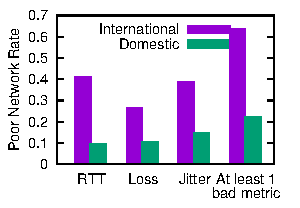
\includegraphics[width=0.45\textwidth]{figures/Via-Opportunity-International.pdf}
        \label{subfig:opportunity-international}
}
\subfloat[\small{Countries of one side of a call}]
{
        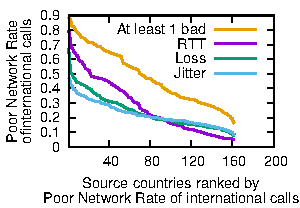
\includegraphics[width=0.45\textwidth]{figures/Via-Opportunity-International-ByCountry.pdf}
        \label{subfig:international-bycountry}
}
\caption{International vs. Domestic Calls.}
\label{fig:country}
\end{figure}

\mypara{International vs. domestic calls} 
On all three network metrics, we see that international 
calls (between users in different countries) have a
 higher PNR, i.e., they are more likely to suffer from 
 bad network performance than domestic calls. 
Figure~\ref{fig:country} shows a $2-3\times$ higher 
PNR on international calls than on domestic calls. 
The figures also show the fraction of calls with at least 
one metric being poor (the last pair of bars), where the 
gap between international and domestic calls is even 
larger. 
Though conclusively diagnosing the root cause of bad 
performance on international calls is hard and beyond 
the scope of this work, the higher PNR for international 
calls points to the WAN path as the culprit.\footnote{One 
aspect is that users tend to use VoIP 
regardless of its performance for international calls, 
unlike domestic calls.} %\cmrvnp{we speculate that it is because ISPs have less incentive to ensure good quality for international calls than domestic ones.}}

% \vnp{The "at least 1 bad metric" bars seem at least as tall as the other bars stacked up, which suggests that there is little overlap between the subsets for which each metric is poor.}

To understand this further, 
Figure~\ref{subfig:international-bycountry} zooms into 
the international calls and classifies them by the country 
of the callers (source). 
We see that there is a skewed distribution, with certain 
countries having a PNR as high as on the individual metrics. 
The PNR of international calls across the remaining 
countries drops gradually but half of them still see a 
non-negligible PNR of $25\%-50\%$. 
This suggests that poor network performance is 
quite widespread, highlighting the suitability of a 
{\em globally} deployed overlay network that provides 
high performance inter-connection between overlay nodes.
% and calling for a selective approach to routing via the managed network. 
% but the overall distribution is flat, indicating that most countries do not have particularly poor network performance. 

\begin{figure}[t!]
\centering
%\hspace{-0.5cm}
\subfloat[Inter-domain vs. intra-domain]
{
        \includegraphics[width=0.45\textwidth]{figures/Via-Opportunity-Interdomain.pdf}
        \label{subfig:opportunity-interdomain}
}%\hspace{-0.5cm}
\subfloat[Source AS]
{
        \includegraphics[width=0.45\textwidth]{figures/Via-Opportunity-Interdomain-ByAs.pdf}
        \label{subfig:interdomain-byas}
}%\hspace{-0.5cm}
\caption{Inter-domain vs. intra-domain calls.}
\label{fig:domain}
\end{figure}

\mypara{Inter-AS vs. intra-AS calls} % The above trends persist when we splice calls by the AS domains of the source and destinations. 
Similar to international calls, calls across ASes 
are $2-3\times$ more likely to experience poor 
network performance than those within the same 
AS domain. %Also, while calls originating from a small fraction of the ASes have a much higher PNR, the overall distribution is even. 
%This, again, points to the need for a selective approach to routing via the global managed overlay.
This, again, points to the need for enabling alternatives to default routing to improve WAN performance.
% a relay system that provides wide-area routing of better performance.

\begin{figure}[t!]
\centering
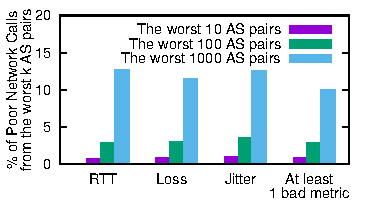
\includegraphics[width=0.6\textwidth]{figures/Via-BadContribution-Top-AsPair.pdf}
\caption{The percentage of calls over poor network 
conditions that come from the worst $n$ AS pairs; 
AS-pairs are ranked in descending order of their 
contribution to total amount of calls with poor performance.}
 %\ga{Change ``top'' to ``worst''.}
\label{fig:bad-contribution}
\end{figure}

\mypara{Not just a few problematic source-destination pairs}
Contrary to our expectation, a few source-destination pairs 
alone do {\em not} account for a big chunk of the PNR. % Our hypothesis was to observe the commonly occurring ``Pareto'' effect.
 Figure~\ref{fig:bad-contribution} shows the fraction of 
 calls that suffer from poor network performance from the 
 worst AS pairs, ranked in order of their contribution to the 
 overall PNR. %Across different metrics, we see that the calls with poor network metrics are not limited to a handful of AS pairs. 
Even the worst $1000$ AS pairs together only count for less 
than $15\%$ of the overall PNR. %\vnp{I'm unable to reconcile these numbers with the bars depicted in Fig 5.} 
This means that localized solutions that fix a few bad ASes 
or AS pairs, e.g., informing the AS administrators or the 
clients directly regarding their ISPs, are not sufficient. 
 
%\vnp{Absolute counts don't quite tell the full story. We should also report what fraction of all AS pairs seen is represented by k}
 
While the above analysis was at the granularity of ASes, 
we also tested at other, finer granularities (e.g., $/24$ and 
$/20$ prefixes of the caller and callee IP addresses) and 
found similar results (of not just a few culprits).
In fact, for the pairs with sufficient data density at the $/24$ 
granularity, we found that performance distributions of the 
network metrics were similar to those at the granularity of ASes.% are close to those at the granularity of $/24$; for instance, on more than 85\% $/24$ pairs where we have at least 10 calls, the average RTT is within 50\% away from that of the corresponding AS pairs.



\begin{figure}[t!]
\centering
%\subfigure[Timeseries\jc{Needs to be changed}]
%{
%        \includegraphics[width=0.45\textwidth]{new-figs/Timeseries-badrate.pdf}
%        \label{subfig:temporal-structure-timeseries}
%}
\subfloat[\small{Persistence}]
{
        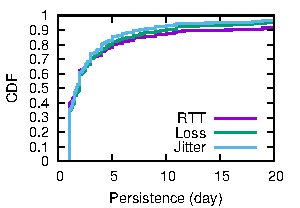
\includegraphics[width=0.45\textwidth]{figures/Via-Persistence-AsPair.pdf}
        \label{subfig:temporal-structure-persistence}
}
\subfloat[\small{Prevalence}]
{
        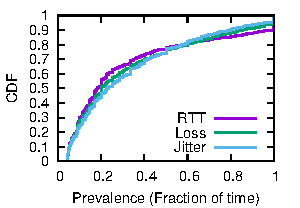
\includegraphics[width=0.45\textwidth]{figures/Via-Prevalence-AsPair.pdf}
        \label{subfig:temporal-structure-prevalence}
}
\caption{Temporal patterns of poor network performance. 
Figure~\ref{subfig:temporal-structure-persistence} and 
\ref{subfig:temporal-structure-prevalence} show the distribution of 
the persistence and prevalence of AS pairs having high PNR.}
\label{fig:temporal-structure}
\end{figure}





\subsection{Temporal Patterns}
\label{subsec:measurement:voip:temporal}

We now analyze temporal patterns of poor network 
performance. 
We perform this analysis by grouping the 
performance of AS pairs into $24$-hour time 
windows.\footnote{Different grouping granularities
yielded similar observations.}
We conservatively label an AS pair as having 
{\em high PNR} for a specific metric (on a given day) if 
its PNR on that day is at least $50\%$ higher than the 
overall PNR of all calls on that day. 

%Knowing what types of calls are more likely to have poor performance, however, does not mean they can be easily fixed. Next, we study the spatial and temporal patterns of bad network performance, and show that fixing a handful of AS pairs in specific time periods does not address most of them, which suggests the needs for a system that can adaptively alleviate bad network performance for users all over the world.

%\myparatight{Methodology} To understand the spatial and temporal patterns of bad network performance, we consider the performance distribution of each AS pair within different time windows of 24 hours. We first group the calls based on the pair of source and destination AS, and to ensure statisical significance, we consider each AS pair that have at least 20 calls in each day\footnote{We decide to group calls by source and destination AS pair on a daily base because it is the finest granularity that still have enough calls for most of the time. We used different grouping granularities and found qualitatively similar observations.}. 
%\ga{Let's see if we can argue for AS-level analysis as reasonable. Maybe present some /24 granularity data, show that the trends are similar when there is sufficient data, and say we will use AS-level data owing to the density? As we have all discussed before, it is not a natural granularity to pick unless we say why so.}

Figure~\ref{subfig:temporal-structure-persistence} and 
\ref{subfig:temporal-structure-prevalence} show the 
distribution of {\em persistence} and {\em prevalence} of 
high PNR AS-pairs. 
The {\em persistence} of an AS pair is the median 
number of consecutive days when it has high PNR. 
The {\em prevalence} of an AS pair is the fraction of 
time it has high PNR.
The figures show a highly skewed distribution with 
$10\%-20\%$ AS pairs always having high PNR, while 
$60\%-70\%$ AS pairs have poor performance for less 
than $30\%$ of time and lasting no longer than one 
day at a stretch. 
%These majority of AS pairs whose poor network performance is neither prevalent nor persistent should be improved in a dynamic manner.
%This means the poor performance of most AS pairs is neither prevalent nor persistent.
%This means that to fix the majority of AS pairs that are neither prevalent nor persistent that statically configuring a solution to improve only the (relatively few) most prevalent and persistent AS pairs is not sufficient; 
This observation suggests that instead of statically 
configuring the system to improve performance for 
only the (relatively few) most prevalent and persistent 
AS pairs, we need to dynamically decide if a call 
should use default Internet routing or be relayed. % sent through overlays.
%It reinforces the point 
%, in order to improve performance for the majority of AS pairs. 


\subsection{Cross-Metric Correlations}
\label{subsec:measurement:voip:correlation}

As there could be dependencies between network 
metrics, improving one metric may increase PNR of another 
metric. 
Figure~\ref{fig:perf-correlation} shows the three pair-wise 
correlations. 
While the plot is based on an aggregation of data across all 
calls and paths, the substantial spread suggests at least the 
possibility that improving one performance metric {\em could} 
lead to a worsening of the other metrics. 
Therefore, we also focus on reducing PNR of three metrics 
collectively, i.e., minimizing how often {\em at least one} of 
the metrics is poor.

\begin{figure}[t!]
\centering
\subfloat[\small{RTT vs. loss rate}]
{
        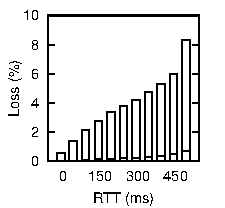
\includegraphics[width=0.3\textwidth]{figures/Via-Quality-Correlation-RTT-loss.pdf}
        \label{subfig:}
}
\subfloat[\small{RTT vs. jitter}]
{
        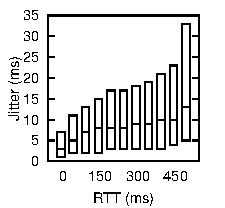
\includegraphics[width=0.3\textwidth]{figures/Via-Quality-Correlation-RTT-jitter.pdf}
        \label{subfig:}
}
\subfloat[\small{Jitter vs. loss rate}]
{
        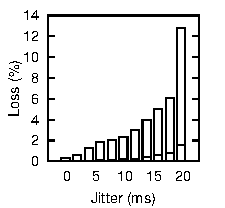
\includegraphics[width=0.3\textwidth]{figures/Via-Quality-Correlation-jitter-loss.pdf}
        \label{subfig:}
}
\caption{Pair-wise correlation between performance metrics. 
The Y-axis shows the distribution ($10^{\text{th}}$, $50^{\text{th}}$, 
$90^{\text{th}}$ percentiles) of one metric as a function the other 
metric over the same set of calls.}
%\ga{Only 25th, median, 90th? Also jitter vs. loss}
\label{fig:perf-correlation}
\end{figure}




%\subsection{Discussion}
%%\subsection{Key Observations}
%\label{subsec:measurement:voip:discuss}
%
%The key observations from this section are:
%\begin{enumerate}
%\item {\em Network performance matters.} User experience of 
%calls is impacted by even small changes in network metrics. 
%\item {\em Wide-area} communication, such as international 
%and inter-domain calls, are more prone to bad network performance, 
%and have a large room of improvement.
%\item Calls suffering from poor networks are spread {\em spatially} 
%(across ASes) and {\em temporally}. 
%%Most calls with poor network performance are not from a handful of source-destination AS pairs. And most source-destination pairs only experience high PNR for a relatively short period of time.
%\end{enumerate}

%These observations motivate the need for a network overlay (Observation 1) that provides better paths with a {\em global} footprint of overlay nodes (Observation 2), and the need to choose routes {\em selectively} and {\em dynamically} (Observation 3). 





\section{Summary}
\label{sec:measurement:summary}

In this chapter, we have presented 
empirical studies based on large-scale datasets of video and VoIP QoE 
to shed light on the structures of QoE problems in the wild.
Our findings suggest that in Internet video and Internet telephony,
there are persistent structures 
in the factors that determine QoE.
Our key observations can be summarized as follows:

\begin{itemize}

\item {\em QoE depends on critical spatial structures.}
Most quality problems can be attributed to 
a relatively small fraction of structures.
We observe that in both Internet video and Internet
telephony, bad quality can be attributed to smaller number
of session-level features. For instance, we
see that \criticalclusters of bad video quality only
account for 2-3\% of all \problemclusters.
Note, however, that VoIP quality problems are more 
spatially spread out than video quality problems, because 
VoIP quality depends
on both sides of a call, while the server side of video sessions 
in general has less heterogeneity than the client side.


\item {\em Many quality problems tend to 
persist on timescales of tens of minutes to hours.}
We observe that a substantial fraction of problems
last for multiple hours (even days).
For instance, 60\% of the problem clusters have a median
duration that last more than 2 hours.
Note, however, that both video and VoIP quality problems 
have highly skewed distributions in the prevalence 
and persistence, where some problems are still transit.


%\item {\em Quality today is not idea.} 
%Across multiple application providers, we observe 
%that a substantial fraction of sessions have bad quality. 
%For instance, 5\% video sessions have a
%buffering ratio larger than 10\%, and 15-17\% Skype
%calls have bad network performance in at least one
%of long latency, high packet loss, or high latency jitter.
%
%\item {\em Most quality problems can be attributed to 
%a relatively small amount of persistent patterns.}
%We observe that in both Internet video and Internet
%telephony, bad quality can be attributed to some
%session-level features (e.g., critical clusters in 
%Section~\ref{subsec:measurement:video:temporal}
%and AS pairs in 
%Section~\ref{subsec:measurement:voip:temporal}).
%These quality problems and features are more stable than 
%fluctuation of quality.

\item {\em Quality problems of different metrics are correlated.} Finally, we observed that
quality problems of different metrics are likely to be correlated,
suggesting that, instead of trading one metric for another,
it is possible to improve multiple metrics simultaneously.

\end{itemize}





